\documentclass[12pt, a4paper]{article}
\usepackage[spanish,es-tabla]{babel}
\usepackage[utf8]{inputenc}
\usepackage[T1]{fontenc}
\usepackage{lmodern}
\usepackage{graphicx}

\makeatletter
\newcommand\setItemnumber[1]{\setcounter{enum\romannumeral\@enumdepth}{\numexpr#1-1\relax}}
\makeatother

\title{Arquitectura de Microprocesadores}
\author{Gianfranco Talocchino}
\date{Marzo - Abril de 2022}

\begin{document}
\maketitle

\section{Preguntas orientadoras}
\subsection{Introducción}
\begin{enumerate}
    \item Describa brevemente los diferentes perfiles de familias de 
    microprocesadores/microcontroladores de ARM. Explique alguna de sus 
    diferencias características.
    
    La familia de arquitecturas ARM Cortex esta dividida en tres 
    principales subfamilias.
    
    \begin{itemize}
        \item Cortex A (\emph{\textbf{A}pplication}): Es la que ofrece mayor rendimiento. Está 
        orientada la ejecución de sistemas operativos como \emph{Linux} y derivados. Su 
        aplicación principal son computadoras, celulares, \emph{tablets}, etc.
        \item Cortex R (\emph{\textbf{R}eal-Time}): Esta orientada y optimizada a aplicaciones 
        \emph{real-time}. Su aplicación se centra en la industria médica, aeronáutica, etc.
        \item Cortex M (\emph{\textbf{M}icrocontrollers}): Esta orientada al uso en 
        microcontroladores y sistemas embebidos de propósito general.
    \end{itemize}
\end{enumerate}
\subsection{Cortex M}
\begin{enumerate}
    \item Describa brevemente las diferencias entre las familias de procesadores Cortex M0, M3 
    y M4.
    
    A grandes rasgos la diferencia es el costo, la velocidad y el consumo de energía. Los 
    Cortex M0 están optimizados para ocupar la menor cantidad de silicio y ser lo mas baratos 
    posible. Frente a los Cortex M3 las diferencias a nivel de Hardware se traducen en
    que algunos core peripherals son opcionales, una arquitectura de memoria Von Neumann y la 
    falta de MPU. Por otro lado, los Cortex M4 añaden la posibilidad de contar opcionalmente 
    con una FPU e instrucciones de DSP. De esta manera, entre los Cortex M0 y M4 el rendimiento
    es creciente, asi como también el costo y el consumo de energía debido a la mayor cantidad 
    de features implementadas en hardware.
    
    \item ¿Por qué se dice que el set de instrucciones Thumb permite mayor densidad de código?
    Explique.
    
    El set de instrucciones Thumb permite mezclar instrucciones de 16 y 32 bits sin que exista una 
    sobrecarga asociada al cambio. Esto da lugar a que operaciones mas simples puedan ser llevadas 
    a cabo con instrucciones de 16 bits en vez de 32 bits. Como resultado, se logra 
    una mayor densidad de código que al solo utilizar instrucciones de 32 bits para operaciones 
    simples y complejas.
        
    \item ¿Qué entiende por arquitectura load-store? ¿Qué tipo de instrucciones no posee este
    tipo de arquitectura?
    
    Una arquitectura de hardware load-store es aquella que solo las instrucciones load y store 
    acceden a memoria RAM. El resto de operaciones (aritméticas, lógicas, etc ..) usan solo 
    registros internos del procesador.
    
    \item ¿Cómo es el mapa de memoria de la familia?
    Los Cortex M tiene un sistema de memoria con direcciones de 32 bits que
    generan un espacio de lineal de direcciones de 4GB. El cual, está participando en 
    número de regiones asignados a diferentes usos. En la Figura \ref{fig:map} se muestra
    un ejemplo.
    \begin{itemize}
        \item Código de programa
        \item RAM
        \item Periféricos
        \item Registros de control
    \end{itemize}
    
    \begin{figure}[!ht]
        \centering
        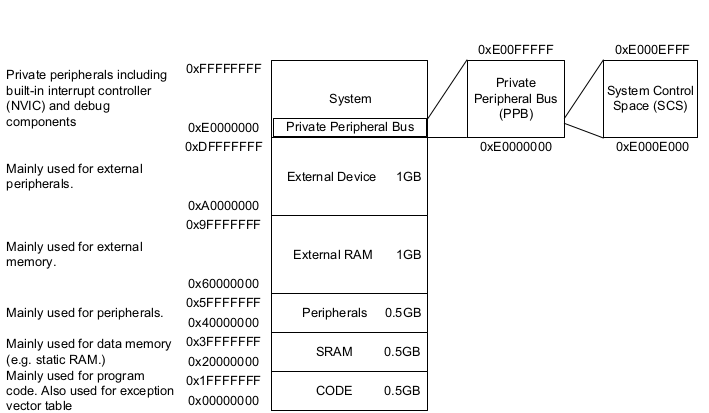
\includegraphics[scale=0.6]{map}
        \caption{Mapa de memoria de la familia Cortex M.}
        \label{fig:map}
    \end{figure}
    
    \setItemnumber{7}
    \item ¿Qué se entiende por modelo de registros ortogonal? Dé un ejemplo
    
    Se dice que una arquitectura de hardware posee un modelo de registros ortogonales 
    cuando el conjunto de instrucciones no impone la limitación de que una cierta instrucción
    deba utilizar exclusivamente un registro especifico. La arquitectura ARM Cortex M posee
    modelo de registros ortogonales. Otras arquitecturas como x86 no.
    
    \setItemnumber{12}
    \item ¿Qué entiende por ``core peripherals''? ¿Qué diferencia existe entre estos y 
    el resto de los periféricos?
    
    Se entiende por ``core peripherals'' a aquellos periféricos que son específicos del 
    procesador, en este caso, procesadores de la familia Cortex M. Se diferencian de los 
    periféricos añadidos por los fabricantes de microcontroladores en que estos son provistos 
    por ARM. El resto, si bien puede agregar las mismas funcionalidades su implementación y capacidad
    variarán notablemente entre fabricantes. Algunos ejemplos de core peripherals para ARM Cortex M 
    incluyen el NVIC, el SysTick, la MPU.
    
    \setItemnumber{14}
    \item ¿Qué es el CMSIS? ¿Qué función cumple? ¿Quién lo provee? ¿Qué ventajas aporta?
    
    El estándar llamado Common Microcontroller Software Interface Standard (CMSIS) desarrollado por 
    ARM es un capa de abstracción para microcontroladores Cortex M. Se encargar de definir interfaces
    para acceso al hardware genérico que estos comparten. Entre las ventajas que aporta se encuentran:
    
    \begin{itemize}
        \item Reduce la curva de aprendizaje del programador.
        \item Reduce los costos de desarrollo.
    \end{itemize}
    
    \setItemnumber{17}
    \item ¿Qué es el systick? ¿Por qué puede afirmarse que su implementación favorece la portabilidad 
    de los sistemas operativos embebidos?
    
    Systick es simplemente un timer presente dentro los microcontroladores basados en ARM Cortex M. 
    En sistemas operativos de tiempo real se usa como temporizador del planificador de tareas. Al estar
    definido por ARM y no variar de un fabricante de microcontrolador a otro facilita
    su portabilidad. Esto ocurre ya que no se necesita cambiar esta fuente de temporización 
    constantemente cuando se pasa de un microcontrolador a otro.
    
\end{enumerate}

\end{document}

